% -*-coding: utf-8 -*-

% Vývoj GPU
% Programovací prostředí
    % CUDA
% Architektura GPU (NVIDIA)
    % Hierarchie paměti
    % Hierarchie paralelizace


%čím rychlejší chceme výpočty, tím více omezneí musíme splnit

%Zatím to vypadá, že klasické qsorty atd. budou mít velké overheady
%Zkusit qsort po warpech a porovnat s tím O(n2), co mám teď, ten taky zjemnit na warpy
%Obecně naplnit sdílenou paměť, něco jako pár threadů na pixel

%    -- je to porovnání s 350 na jeden krok CC porovnání s 32 v jednom z několika kroků + scan sumy

%BES na CPU (rozkrájený quickselect)

V této kapitole se stručně seznámíme s historií a vývojem v oboru výpočtů na GPU, rozebereme vlastnosti, přednosti a nevýhody GPU architektury v porovnání s klasickým CPU a nakonec popíšeme programovací model CUDA\footnote{Compute Unified Device Architecture} od společnosti NVIDIA, který použijeme pro implementaci filtrů na GPU.

\section{Vývoj GPU}

    S použitím GPU pro jiné, než grafické výpočty se začalo experimentovat, jakmile přestaly být grafické karty -- hlavně díky rozvoji herního průmyslu -- pouhým jednoúčelovým zařízením a staly se z nich, alespoň částečně, programovatelné paralelní procesory. Vzhledem k tomu, že karty byly primárně určené ke zpracování grafiky, daly se výpočty provádět pouze pomocí grafického API například přes textury a programovatelné pixel-shadery, což značně snižovalo efektivitu zpracování díky vysoké režii API.

    Zřejmě první velká společnost, která se rozhodla vyjít vstříc požadavkům na konstrukci GPU jako univerzálně použitelné vysoce paralelní výpočetní jednotky, byla NVIDIA, když změnila celý koncept nově vyvíjeného čipu a zavedla tzv. CUDA-jádra -- obecnější a pružnější, než jednotky dedikované ke specifickým grafickým operacím\footnote{ty jsou ovšem na kartách stále přítomny a lze je v programu pro tyto specifické operace použít (např. výpočet $\sin$, $\cos$)}. V únoru 2007 pak představila první verzi vývojového nástroje CUDA, který umožňoval efektivně využívat hardware GPU pomocí několika rozšíření jazyka C a posléze \Cpp. CUDA-jádra novějších karet dokonce umí počítat nativně v dvojnásobné přesnosti; u běžných karet jsou ale tři čtvrtiny jader pro dvojitou přesnost deaktivovány \cite{Heller} (pro grafické operace nejsou třeba), a pro plný výkon ve dvojité přesnosti si musíme koupit (řádově dražší) kartu ze série TESLA, která je primárně určena pro intenzivní výpočty. Veškerý vývojový software poskytuje NVIDIA zdarma.

    V současnosti existují k CUDA dvě alternativy: prostředí OpenCL\footnote{Open Compute Language}, zaštítěné sdružením Khronos Group, které se profiluje jako standard pro heterogenní paralelní programování a DirectCompute od Microsoftu stojící na balíku DirectX verze 10 a vyšší. Výhodou OpenCL je, že stejný kód lze zkompilovat jak pro CPU, tak pro GPU výrobců ATI a NVIDIA\footnote{jinak se bohužel jedná o vzájemně nekompatibilní technologie}. Z principu tedy nemůže poskytovat tak pohodlný přístup, jako CUDA a výsledkem je poměrně rozsáhlý kód. \emph{Dále se budeme zabývat pouze prostředím CUDA a hardwarem s ním souvisejícím.}

    \subsection{Současnost}

     V současnosti je GPGPU\footnote{General Purpose computation on Graphics Processing Units} již etablovaný obor. Hlavní trend vývoje GPU je nyní podobný, jako v počátcích CPU -- spočívá v odstraňování omezení, která musíme na kód klást, abychom dosáhli optimálního výkonu, a ve větší univerzalizaci hardwaru. Tím pádem se i~rozšiřuje množina úkolů vhodných pro zpracování na GPU. Jednotlivé výpočetní jednotky na kartách už dávno nejsou pouhými jednoduchými vektorovými procesory, ale stále více se blíží plnohodnotnému (vícejádrovému) procesoru, i když si samozřejmě svůj vektorový charakter zachovávají. Asi nejvíce je to vidět na práci s pamětí, kde u nejnovějšího čipu \FERMI ~z dílny NVIDIA přibyla vrstva cache, čímž se zmenšila omezení přístupu do globální paměti (viz dále), ale došlo i k rozdělení vektorového procesoru na dva téměř samostatně fungující díly \cite[přílohy]{CUDA programming g.}.

\section{Architektura GPU}

    \subsection{Rozdíly CPU a GPU}

        Nyní se podrobněji podíváme na specifika architektury čipů grafických karet. Hlavní otázkou je, pro jaké úlohy jsou vůbec GPU vhodné. Obrázek~3.1 zhruba ukazuje, jak velká část čipu (DRAM ovšem není přímo na čipu) CPU a GPU je dedikována pro určitý druh operací.

        \begin{figure}[h]
          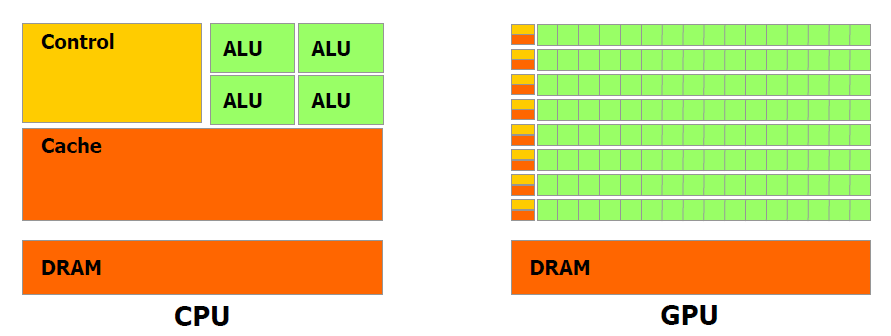
\includegraphics[width = \textwidth]{src/2Gpu/CPUGPU.png}
          \caption{Rozdíly využití čipu na CPU a GPU, převzato z \cite{CUDA programming g.}}
        \end{figure}\label{cpu vs gpu}

        Vidíme, že velkou část čipu CPU zabírá cache a kontrolní logika. Ty zajišťují několika ALU\footnote{Arithmetic Logic Unit} dostatečný přísun dat a instrukcí (např. pomocí hyper-threadingu a branch-prediction), lhostejno jak moc se program větví, nebo jak jsou data uspořádána v DRAM.

        GPU se naproti tomu skládá z několika samostatně funkčních vektorových procesorů -- tzv. SM\footnote{Streaming Multiprocesor} jednotek, z nichž každá má vlastní malou cache a z kontrolní logiky má naprosté minimum. Z toho plyne jednak jistá nutná disciplína při přístupu do DRAM, která je ale narozdíl od té na CPU lépe optimalizovaná na sekvenční čtení, a za druhé musíme běh programu přizpůsobit tomu, že GPU je po částech SIMD\footnote{Single Instruction Multiple Data}, respektive SIMT\footnote{Single Instruction Multiple Thread -- název pocházející od NVIDIA} -- narozdíl od vícejádrového CPU, které je plnohodnotné MIMD\footnote{Multiple Instruction Multiple Data}. Podrobný popis nejnovějšího SM z čipu \FERMI ~lze nalézt v \cite{Fermi}.

        Obecně můžeme říci (protože velká část čipu GPU je dedikována pro aritmetiku), že GPU je nejvíce vhodná pro aritmeticky intenzivní výpočty, tzn. mající vysoký poměr počtu aritmetických operací ku počtu přístupů do paměti.

    \subsection{Algoritmy vhodné pro GPU}

        Před paralelizací algoritmu pro GPU musíme tedy zvážit, zda to má vůbec smysl -- pro dosažení optimálního urychlení musí algoritmus v co největší míře splňovat následující body:
        \begin{itemize}
          \item rozložitelnost výpočtů na nezávislé části, které lze vykonávat paralelně (výsledek jedné nezávisí na výsledku ostatních)
          \item nutná omezená nebo žádná komunikace s CPU
          \item malý počet přístupů do paměti, nejlépe sekvenční/blokové
          \item podobný kód ve všech paralelních částech, minimální a předvídatelné větvení programu
        \end{itemize}

        Jak uvidíme, filtrování obrazu nesplňuje tyto body úplně (např. přístupy do paměti) -- kdyby splňovalo vše, tak se jím nemá příliš cenu zabývat -- ale dostatečně na to, abychom dosáhli použitelných výsledků.

\section{Pogramovací model CUDA a jeho HW implementace}

    \subsection{Úvod}
    Pro maximální efektivitu paralelizace vyvinula NVIDIA několikavrstvou dobře škálovatelnou strukturu s přímou návazností na svůj hardware. Nejmenší výpočetní jednotkou z pohledu programu je \emph{vlákno} (thread), který fyzicky běží na jednom CUDA-jádře v SM. Vlákna se sdružují do \emph{bloků}, které běží na celém SM a mohou mít 1D, 2D, nebo 3D strukturu, podle toho jakého charakteru jsou zpracovávaná data. Poslední článek tvoří \emph{grid} běžící na celé GPU obsahující (zatím) nejvýše 2D strukturu bloků. Z programu pak výpočty spouštíme pomocí volání \emph{kernelu} obsahujícího náš kód, kterému sdělíme v kolika blocích má běžet, jakou mají mít strukturu v gridu, kolik vláken má být uvnitř bloku a jak mají být uspořádány. To umožňuje ten samý kernel spouštět na různých zařízeních, protože sám hardware rozhoduje, jak jednotlivé výpočetní elementy mezi SM (a posléze CUDA-jádra) rozdistribuuje.

    \subsubsection{Úrovně přístupu}

    Na straně uživatele poskytuje NVIDIA dvě rozhraní: nízkoúrovňové CUDA Driver API a vysokoúrovňové CUDA runtime API, v současnosti ve verzi 4.0. Driver API poskytne uživateli totální kontrolu nad kartou výměnou za složitější a delší kód -- uživatel musí zajistit inicializaci zařízení, přesun dat a funkčních parametrů pro kernel na kartu a přesun a spuštění kernelu samotného. Rozhraní Driver API je v C a funkčně zhruba odpovídá OpenCL. Runtime API je rozšířením C, které umožňuje kernel napsat podobně jako funkci v C a při volání jí speciální syntaxí sdělit, kolik vláken a bloků chceme spustit. O inicializaci a vše ostatní se postará runtime. Používání více GPU z jednoho procesu na CPU umožňuje až nejnovější verze CUDA 4.0 (v době psaní kódu byla k dispozici pouze CUDA 3.2).

    Mixování obou přístupů (např. právě kvůli použití více zařízení) se nedoporučuje, ale v rozumné míře možné je -- pravidla mixování stanovila opět až CUDA 4.0. V našem kódu používáme výhradně Runtime API, proto se dále budeme zabývat pouze jí.

    \subsubsection{Výpočetní schopnost}

    Tento termín bude dále v textu často používán. Výpočetní schopnost\footnote{Compute Capability} (CC) udává fyzickou verzi čipu -- všechna CUDA-enabled zařízení před architekturou \FERMI ~mají CC 1.x, čipy s touto architekturou 2.x. Různé CC se liší množsvím paměti, registrů, strukturou SM atd. Největší skok je samozřejmě mezi 1.x a 2.x. Podrobný popis rozdílů mezi CC je k dispozici v \cite[přílohy]{CUDA programming g.}. Pokud budeme dále uvádět konkrétní hodnoty, budou pro CC 1.0, pro kterou je kód primárně optimalizován. Pokud to bude důležité, bude v závorce uvedena hodnota pro CC 2.0.
    
    \vspace{0.5cm}
    
   \emph{Experimentální výpočty byly prováděny na kartě 8800 GTX s CC 1.0, neboť pouze ta byla v danou chvíli nejlépe k dispozici. V textu však budeme přesto zmiňovat i hodnoty a vlatnosti týkající se vyšších CC a diskutovat jejich možný přínos. Vzhledme k tomu, že testovací CPU je podobného stáří jako karta, považujeme výsledky za zcela průkazné.}

    \subsection{Kernel}

    Runtime API nám dovoluje míchat kód pro CPU i GPU v jednom souboru, definici kernelu proto rozlišíme specifikátorem
    \Vr"\cy{__global__}" (příklad převzat z \cite{CUDA programming g.}).

    \begin{Verbatim}[commandchars = \\\{\}]
    // definice kernelu
\cy{__global__} \bl{void} MyVecAdd(\bl{float} *A, \bl{float} *B, \bl{float} *C)\{
    \bl{int} i = \cy{threadIdx}.x;
    C[i] = A[i] + B[i];
\}
    // volání kernelu v programu
    MyVecAdd<<<1,N>>>(A,B,C);
    \end{Verbatim}

    Při volání v příkladu specifikujeme, že chceme jeden blok a N vláken jako vektor, vektory A, B a C musí být při volání již připraveny v paměti karty. Po spuštění dostane každé vlákno (potažmo blok) své ID, které je v kódu přístupné přes konstantní proměnnou \Vr"\cy{threadIdx}" (potažmo \Vr"\cy{blockIdx}") a umožní tak diferenciaci vláken. V kernelu tedy píšeme kód \emph{jediného vlákna}, jehož konkrétní chování se po spuštění \emph{odvíjí od přiděleného ID námi definovaným způsobem}.

    \subsection{Hardwarová paralelizace, multithreading}

    Zde popíšeme, co se skutečně děje při spuštění kernelu na GPU. Přitom se omezíme pouze na jeden SM, protože všechny SM na kartě pracují zcela nezávisle a jakákoliv jejich synchronizace v rámci jednoho kernelu není možná.

    Po spuštění kernelu se bloky rozdistribuují mezi jednotlivé SM. Kolik bloků se vejde současně na jeden SM je dáno tím, kolik registrů a sdílené paměti blok spotřebuje -- tyto hodnoty jsou pevně stanoveny při spuštění kernelu. Pokud se na SM nevejde ani jeden blok, spouštění kernelu selže. V opačném případě hardware umístí na každý SM maximální možný počet bloků, zbývající bloky budou čekat na uvolnění některého SM.

    SM má však pouze 32 CUDA-jader, tzn. bloky běží současně pouze virtuálně. Důvod tohoto \bq přesycení\eq~ spočívá v \emph{překrytí latencí} způsobených například čtením a zápisem do paměti: pokud například nějaký \emph{warp} (což je 32 synchronně běžících vláken na oněch 32 CUDA-jádrech) čeká na načtení operandů z paměti, může mezitím jiný warp (protože má např. proměnné připravené v registrech) provádět výpočty -- i když je to třeba warp z jiného bloku. Rychlé přepnutí warpů\footnote{tzv. context switch} je umožněno tím, že vlákno na GPU je narozdíl od toho na CPU velmi jednoduchá struktura a multithreading na GPU je dělán hardwarově. Z toho vyplývá jisté omezení na maximální počet bloků a vláken/SM (přesná čísla lze nalézt v \cite{CUDA programming g.}). Ve většině případů ovšem dříve vyčerpáme registry, nebo sdílenou paměť, než se dostaneme k tomuto stropu.

    Pro efektivní využití výpočetních jednotek je nutné, aby pokud možno všechna vlákna v jednom warpu prováděla stejný kód, neboť celý warp zvládá naráz vykonávat pouze jedinou instrukci (dvě instrukce pro dva 16vláknové půlwarpy pro CC 2.x), což odpovídá filozofii SIMD. Všechna větvení kódu by tedy měla být směřována na hranice warpů, tzn. mezi 32 po sobě jdoucích vláken. V opačném případě bude warp rozdělen na části se stejnou posloupností instrukcí a ty budou zpracovány sériově.

    \subsection{Práce s pamětí}

    Jak jsme zmínili v úvodu kapitoly, paměťové zdroje karet jsou poměrně omezené a vhodné zacházení s pamětí je tak prvním předpokladem pro to, aby paralelizovaný algoritmus dosáhl optimálních výsledků. Vývoj jde ale v této oblasti hodně dopředu a architektura \FERMI ~má již paměti mnohem více a lépe strukturované.

    \subsubsection{Registry}

     GPU ragistry jsou velmi podobné klasickým registrům na CPU a jsou zdaleka nejrychlejší pamětí dostupnou pro vlákno -- proto se do nich ukládají všechny lokální proměnné kromě polí. Karty s CC 1.x mají 8192 (1.0) až 16384 (1.3) registrů/SM, CC 2.x má 32768 registrů/SM. V kódu není třeba je nějak značit, většina lokáních proměnných (viz dále) se do nich sama uloží.

    \subsubsection{Sdílená paměť}

    Jedná se o paměť zabudovanou v každém SM, dostupnou na úrovni bloku a umožňující komunikaci vláken v bloku (u CC 2.x se jí část dá vyhradit pro cacheování přístupů do globální paměti). Hardwarově se jedná o SRAM\footnote{Static Random Access Memory}, je přímo na čipu GPU a tudíž je poměrně rychlá. Pro optimální rychlost je rozdělena do 32 banků tak, že vlákna (jednoho warpu) čtoucí 32 po sobě jdoucích položek z pole v této paměti přistupují každé do jednoho banku a celé čtení je možné vyřídit jako jedinou operaci.

    V kódu statické pole pevné délky ve sdílené paměti deklarujeme pomocí identifikátoru \Vr"\cy{__shared__}" -- takto je definováno jedno pole pro celý blok (obyčejná proměnná bez identifikátoru by byla vytvořena pro každé vlákno) a všechna vlákna bloku do něj mají přístup. Synchronizace čtení a zápisu je ponechána na uživateli.

    Pole ve sdílené paměti je možné alokovat i dynamicky z CPU: v kernelu ho deklarujeme pomocí identifikátoru \Vr"\bl{extern}":
    \begin{Verbatim}[commandchars = \\\{\}]
\bl{extern} \cy{__shared__} \bl{datovýtyp} jménopole[];
    \end{Verbatim}
    Při spouštení kernelu poté pomocí třetího parametru {\tt Ns} zadáme, kolik chceme navíc (kromě režie) alokovat bytů sdílené paměti pro blok.
    \begin{Verbatim}[commandchars = \\\{\}]
MyKernel<<<1,N,Ns>>>(parametry);
    \end{Verbatim}
    Námi deklarované pole se naváže na začátek této alokované paměti. Nevýhodou je, že při deklaraci více dynamicky alokovaných polí budou všechny začínat na začátku této paměti (jako v unii) a případné rozdělení pole musíme tedy provést ručně pomocí ukazatelů a offsetů. Dynamická alokace přímo z vlákna není principiálně možná. Životnost dat ve sdílené paměti je stejná jako životnost bloku.

    \subsubsection{Globální paměť}

    Jedná se o největší paměť na GPU (jednotky GB). Protože není fyzicky umístěna na čipu, přístup do ní je velmi pomalý -- řádově stovky taktů -- nicméně je optimalizová pro sekvenční čtení a zápis z GPU. Hardware umožňuje přístup pouze po 128-bytových blocích -- pokud nechceme, aby došlo ke zpomalení, je nutné, aby všechna vlákna v jednom warpu (a tudíž vykonávající stejnou instrukci) přistupovaly do co nejmenšího počtu těchto bloků, ideálně do jednoho. Tím dojde k tzv. \emph{sdruženému přístupu}\footnote{Coalesced access} a všechny přístupy vláken do sousedících míst v paměti mohou být obslouženy v rámci jediného požadavku. Konkrétní způsob (omezení), jak mohou vlákna k paměti v bloku přistupvat, je závislý na výpočetní schopnosti karty a jeho popis lze nalézt v \cite{CUDA programming g.}.

    Alokace, čtení a zápis do této paměti je možný i z CPU (samozřejmě na jiné bázi), data zapsaná tímto způsobem mají pak životnost stejnou, jako aplikace.

    V kódu se ukazatel do globální paměti neliší od jiných ukazatelů\footnote{K dispozici je i \bq novější\eq ~obecný typ ukazatele do globální paměti {\tt DevicePtr*}, který vyžadují nekteré fukce. Spíše jde ale o snahu nějak data na CPU a GPU formálně oddělit. Kód využívající tento typ ukazatele se nám však nepodařilo zprovoznit. Se starší verzí jsou však dobré zkušenosti.}, postup zkopírování dat na GPU je následující:
    \begin{enumerate}
      \item Vytvoření běžného ukazatele na požadovaný typ na CPU
      \item Přiřazení ukazatele k alokovanému poli v globální paměti pomocí {\tt CudaMalloc(...)}
      \item Zkopírování dat z pole v RAM na GPU pomocí {\tt CudaMemcpy(...)}
      \item Předání ukazatele kernelu přes obyčejný parametr
    \end{enumerate}
    Na CPU nelze ukazatel do globální paměti dereferncovat přímo, na GPU to však lze bez jakýchkoliv omezení.

    Samotnou alokaci opět není možné provádět z GPU, pokud však využívá vlákno větší statické pole jako lokální proměnnou, nebo tolik proměnných, že se nevejdou do registrů\footnote{tzv. Register spilling}, uloží se přebytek v \emph{lokální paměti}. Lokální zde znamená pouze omezení životnosti dat, data jsou ve skutečnosti uložena do globální paměti -- se všemi nevýhodami, které z toho plynou. Z tohoto důvodu je dobré se použití lokální paměti jakýmkoliv způsobem vyhnout.

    \subsubsection{Konstantní paměť}

    Konstatntní paměť je 64 KB velká část globální paměti s vlastní cache, tudíž je celkem rychlá a vhodná pro objemné konstanty. Je přístupná z CPU pro čtení i zápis, dynamická alokace není možná ani z CPU. Z GPU lze paměť pouze číst -- proto konstatní.

    V kódu se pro tuto paměť používá identifikátor \Vr"\cy{__constant__}" a proměnné s tímto identifikátorem musíme chápat spíše jako pevné přidělení místa v konstantní paměti karty na úrovni aplikace. Poněkud nepříjemné je, že z tohoto důvodu musí být všechny tyto proměnné v kódu definovány jako globální a na úrovni souboru. Nesmí být tedy schovány do jakéhokoliv prostoru jmen, ani do třídy (byť jako statické), jak je zvykem ve slušném \Cpp ~kódu. Hodnoty do proměnných (polí) v konstantní paměti přesuneme z RAM pomocí {\tt CudaMemcpyToSymbol(...)}.

    \subsubsection{Texturová paměť}

    Texturová paměť někdy představuje rychlejší alternativu k čtení (\emph{nikoliv zápisu}) z globální paměti. Část dat můžeme totiž prohlásit za \emph{texturu}, což znamená, že data budou každým SM částečně cacheována. Velikost cache je 6-8 KB/SM, přitom hardware sám odhaduje, která data bude chtít program načíst a ty do ní přesune\footnote{tzv. Texture fetching}. Pokud jsou požadována data, která nejsou v cache k dispozici\footnote{tzv. Cache miss (v opačném případě Cache hit)}, jsou normálním způsobem načtena z globální paměti. Používání textur je tedy výhodné, pokud bloky potřebují relativně malé a dobře definované kousky dat, které se do cache vejdou celé.

    Protože se jedná o činnost hodně blízkou klasické grafice, je v kódu citelně znát odkaz grafického API. Před použitím textury musíme definovat referenci na texturu (opět globální stejně jako konstantní proměnné) a ještě na CPU ji svázat s požadovanými daty pomocí {\tt cudaBindTexture(...)}. Obě operace potřebují značné množství parametrů (potřebných při používání textur pro původní účel), jejich popis lze nalézt v~\cite{CUDA programming g.}. Číst z takto připravené textury je na GPU možné pomocí funkce {\tt texXDfetch(...)} ({\tt X} je 1,2,3).

    CC 2.x již umožňuje volitelné cacheování globální paměti za použití části sdílené paměti, textury ale stále představují průchozí alternativu. Nezaberou totiž sdílenou paměť a využijí několik cenných KB paměti jinak nepoužívané.

    \subsection{Možnosti synchronizace}

    Synchronizace vláken je nutná pro jakoukoliv jejich kooperaci mezi sebou. CUDA umožňuje synchronizaci na úrovni bloku pomocí instrukce \Vr"\cy{__syncthreads()}", která zastaví běh vláken, dokud všechna v jednom bloku tuto instrukci nezavolají. To se hodí například při práci se sdílenou pamětí, kdy chceme zajistit, aby z ní všechna vlákna začala číst až poté, co do ní budou (např. menším počtem vláken) zapsána relevantní data.

    CUDA navíc poskytuje i několik speciálních instrukcí čistě pro synchronizaci přístupů do paměti (viz \cite[přílohy]{CUDA programming g.}), což je jediná možnost, jak částečně synchronizovat vlákna v celé aplikaci -- ovšem za cenu výrazného zpomalení (poruší se přepínání bloků na SM kvůli překrývání latencí).

% v implementaci chceme už jen popisovat optimalizace, programming model už musí být hotový 